\subsection{Соединения элементов 13 группы, способы получения, химическое поведение, электронное и геометрическое строение молекул}

\subsubsection*{B}

\textbf{Получение}

1) Пиролиз бороводородов

$$B_2H_6 \rightarrow B + H_2$$

2) Металлотермия

$$B_2O_3 + Mg \rightarrow MgO + B$$

3) Получение кристаллического бора

$$BBr_3 + H_2 \xrightarrow{W, 1000^{\circ}} B + HBr$$

\textbf{Химические свойства}

1) Химически инертен, при н.у.  не раегирует с $H_2O, H^+, OH^-$

2) С неметаллами

$$B + O_2 \xrightarrow{700^{\circ}} B_2O_3$$
$$B + Cl_2 \xrightarrow{800^{\circ}} BCl_3$$
$$B + F_2 \rightarrow BF_3$$
$$B+ N_2 \xrightarrow{900^{\circ}} BN$$


3) Аморфный B активнее кристаллического, окисляется кислотами-окислителями и в $OH^-$-расплавах

$$B + HNO_{3(konc)} \xrightarrow{100^{\circ}} H_3BO_3 + NO_2$$
$$B + KClO_3 + KOH \rightarrow KBO_2 + KCl + H_2O$$

4) При высокой температуре ($>1000^{\circ}$) с оксидами

$$B + H_2O \rightarrow B_2O_3 +H_2$$
$$B + P_2O_5 \rightarrow P_4 + B_2O_3$$

\textbf{Строение}

1) В основе кристаллического строения B лежит икосаэдр $B_{12}$

2) 2 стабильных изотопа ${^{10}B}, {^{11}B}$

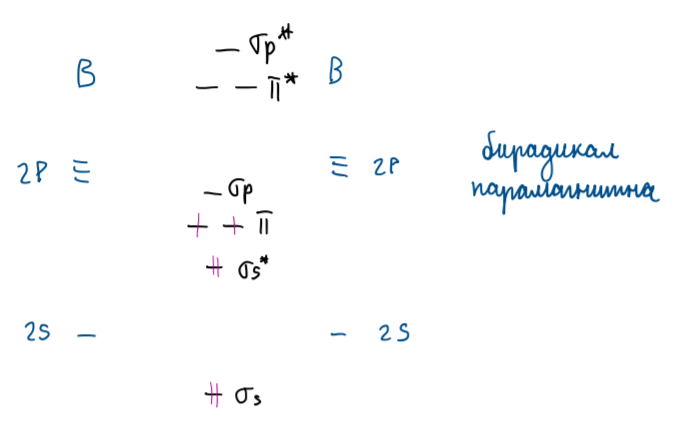
\includegraphics{images/11v1.png}

\subsubsection*{Al}

\textbf{Получение}

$$Al_2O_3 \xrightarrow{Na_3AlF_6} Al + O_2$$
(на графитовых электродах)

$$AlCl_3 + K \rightarrow KCl + Al$$

\textbf{Химические свойства}

1) С кислотами-неокислителями ($HCl, H_2SO_{4(razb)},..$)

2) С киcлотами-окислителями при нагревании, т.к. идет пассивация
($HNO_3, H_2SO_4$ - обе концентрированные)

3) С $OH^-$

$$Al + NaOH + H_2O \rightarrow Na[Al(OH)_4] + H_2$$
$$Al + NaOH \rightarrow Na_2O + NaAlO_2 +H_2$$

4) Алюминотермия

$$Al + Fe_3O_4 \rightarrow Fe + Al_2O_3$$
$$ Al + Cr_2O_3 \rightarrow Cr + Al_2O_3$$

5) С неметаллами

$$Al + O_2 \rightarrow Al_2O_3$$
$$Al + X_2 \rightarrow AlX_3 (X=Cl,Br, I)$$

При нагревании с $F_2, S, N_2, C$

\textbf{Строение}

1) В возбужденном состоянии способен отдавать все 3 электрона $\Rightarrow$ характерна с.о +3

2) Плотнейшая кубическая решетка типа Cu, КЧ =12

\subsubsection*{Ga, In, Tl}

\textbf{Получение}

1) Электролиз водных растворов солей

2) Ga, In из отходов производства Al и Zn

3) Tl - сопутствует Pb в $S^{2-}$ рудах

\textbf{Химические свойства}

1) В кислотах-неокислителях: Ga, In +3, Tl +1

2) С $OH^-$
$$ Ga + KOH + H_2O \rightarrow K[Ga(OH)_4(H_2O)_2] + H_2$$

3) C неметаллами

$$Tl + S \xrightarrow{230^{\circ}} Tl_2S$$
$$Tl + Cl_2 \xrightarrow{120^{\circ}} TlCl$$

4) С $H_2O$

$$Ga + H_2O \xrightarrow{350^{\circ}} GaOOH + H_2$$
$$In + H_2O \nrightarrow$$
$$Tl + H_2O + O_2 \xrightarrow{50^{\circ}} TlOH$$

\textbf{Строение}

11) Постпереходные элементы

2) $6s^2$ пара Tl понижает стабильность соединений в высшей с.о

3) Есть d- и f- сжатие (Tl)

Ga - слоюная орторомбическая решетка\\
In - тетрагональная решетка, искажение структуры Cu, кч =12\\
Tl - гексагональная структура типа Mg, кч = 12

\subsubsection*{Гидриды}

$B_2H_6$

\textbf{Получение}
$$MgB_2 + Mg + HCl \rightarrow MgCl_2 + B_2H_6$$
$$BF_3 NaH \rightarrow NaF + B_2F_6$$

\textbf{Химические свойства}

1) Гидролиз 
$$B_2H_6 + H_2O \rightarrow H2BO_3 + H_2$$

2) Горение

$$B_2H_6  + O_2 \rightarrow H_3BO_3$$

3) С HX
$$B_2H_6 + HCl \rightarrow B_2H_5Cl + H_2$$

4) С MeH

$$B_2H_6 + LiH \xrightarrow{Et_2O} LiBH_4$$

5) С $NH_3$

$$B_2H_6 + NH_3 \rightarrow B_3H_6N_3$$

6) С галогенами

$$B_2H_6 + Cl_2 \rightarrow BCl_3 + HCl$$

\textbf{Строение}

Гидриды очень разнообразны:

- Клозо-бораны $[B_nH_n]^{2-}$ n=6-12\\
-Нидо-бораны $B_nH_{n+4}$ (в т.ч $B_2H_6$) незакрытые с одной стороны полиэдры\\
-Арахно-бораны $B_nH_{n+8}$ полиэдры с двумя свободными вершинами\\
-Гиозо-бораны $B_nH_{n+8}$ - 3 свободные вершины\\
-Конжукто-бораны  - сложные комбинации типов выше

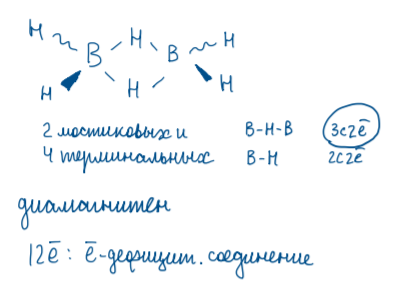
\includegraphics{images/11v2.png}

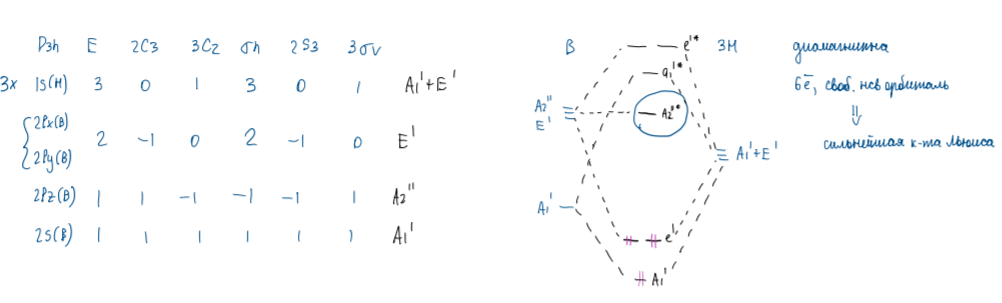
\includegraphics{images/11v3.png}


Тетрагидробораны

\textbf{Получение}

$$B_2H_6 + LiH \rightarrow Li[BH_4]$$

\textbf{Химические свойства}

1) Гидролиз ($Na[BH_4]$ растворим)

$$Li[BH_4] + H_2O \rightarrow LiBO_2 + H_2$$

2) Восстановительные свойства

$$Li[BH_4] + I_2 \rightarrow BI_3 + LiI + H_2$$
$$Li[BH_4] + GeCl_4 \rightarrow GeH_4 + BCl_3 + LiCl$$

\textbf{Строение}

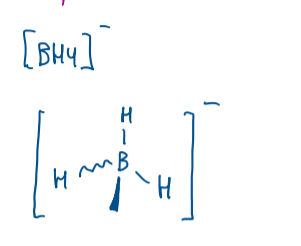
\includegraphics{images/11v4.png}

$Li[AlH_4]$

\textbf{Получение}

$$LiH + AlCl \xrightarrow{Et_2O} LiCl + Li[AlH_4]$$

\textbf{Химические свойства}

$$Li[AlH_4] + H_2O \rightarrow LiOH + Al(OH)_3 + H_2$$

Сильнейший восстановитель

$$Li[AlH_4] + SiCl_4 \xrightarrow{efir} SiH_4 + AlCl_3 + LiCl$$

$$Li[AlH_4]  + H_2SO_4 \rightarrow AlH_3 + H_2 +Li_2SO_4$$

\textbf{Строение}

$Li[AlH_4]$ - из тетраэдр. группировок $AlH_4^-$, соед. мостиковыми атомами Li

$(AlH_3)_n$ - бесконечный полимерный каркас, отктаэдры $AlH_6$ объединены 6-ю связями $Al-H-Al$


$Ga, In, Tl$ - гидриды неустойчивы, а $M'[MH_4]$, где M' - щелочной,  а M = Ga, In, Tl, разлагаются при $0-5^{circ}$\\
Вниз по группе падает устойчивость\\

Например при н.у $Ga_2H_6 \rightarrow Ga + H_2$\\
Химия дигаллана аналогична диборановой

\subsubsection*{Оксиды и кислоты}

$B_2O_3$

\textbf{Получение}

$$B + O_2 \xrightarrow{630^{\circ}} B_2O_3$$
$$H_3BO_3 \xrightarrow{250^{\circ}} B_2O_3 + H_2O$$

\textbf{Химические свойства}

Кислотный оксид со слабыми признаками амфотерности

$$B_2O_3 + P_4O_{10} \rightarrow BPO_4$$

$$B_2O_3 + H_2O \xrightarrow{800^{\circ}} HBO_2$$

$$B_2O_3 + HCl \rightarrow BCl_3 + H_2O$$

$$B_2O_3 + C + Cl_2 \rightarrow BCl_3 + CO$$

$$B_2O_2 + Na_2O_2 \rightarrow NaBO_2 + O_2$$

\textbf{Строение}

Построен из плоских треугольников $BO_3$, соед. общими вершинами в 3D-структуру

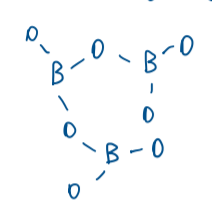
\includegraphics{images/11v5.png}

$H_3BO_3$

\textbf{Получение}

$$Na_2[B_4O_5(OH)_4]\cdot 8H_2O + H_2SO_4 \rightarrow B(OH)_3 Na_2SO_4 + H_2O$$
$$Na_2CO_3 + H_3BO_3 \rightarrow CO_2 + H_2O + Na_3BO_3$$

\textbf{Химические свойства}

1)Слабая одноосновная кислота

$$B(OH)_3 + HOH \leftrightarrows H^+ + [B(OH)_4]^-$$

2) Образование эфиров (окрашивание пламя в зеленый)

$$H_3BO_3 + CH_3OH \xrightarrow{H_2SO_{4(k)}} B(OCH_3)_3 + H_2O$$

3) Частичная дегидратация

$$H_3BO_3 \xrightarrow{>100^{\circ}} (HBO_2)_n$$

\textbf{Строение}

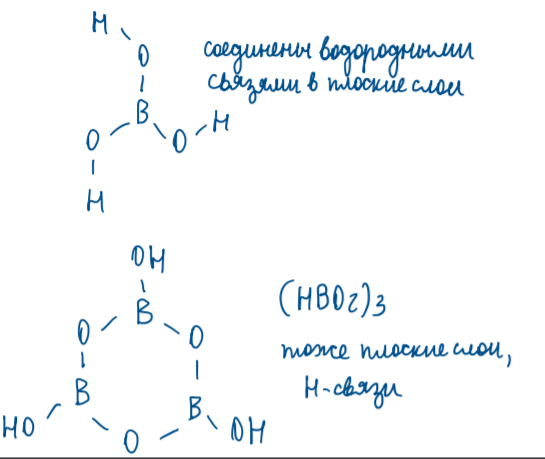
\includegraphics{images/11v6.png}


$H_2B_4O_7$

\textbf{Получение}

1)  Процессы поликонденсации

$$2B(OH)_3 + 2[B(OH)_4]^- \leftrightarrows [B_4O_5(OH)_4]^{2-} + 5H_2O$$

$$HBO_2 \rightarrow H_2B_4O_7 + H_2O$$

2) Только двузамещенные соли ( в растворе только тетрабораны)

$$H_3BO_3 + NaOH \rightarrow Na_2B_4O_7$$

\textbf{Химические свойства}

1) Двухосновная кислота

$$H_2B_4O_7 \rightarrow 2B_2O_3 + H_2O$$

2) Бура

$$Na_2[B_4O_5(OH)_4]\cdot 8H_2O \xrightarrow{61^{\circ}} Na_2[B_4O_5(OH)_4]\cdot 3H_2O \xrightarrow{161^{\circ}} Na_2[B_4O_5(OH)_4]$$

$$Na_2[B_4O_5(OH)_4] \xrightarrow{380^{\circ}} Na_2B_4O_7$$

$$Na_2B_4O_7 + H_2O \rightarrow H_3BO_3 + NaOH$$
$$Na_2B_4O_7 + HCl + H_2O \rightarrow H_2BO_3 + NaCl$$
$$Na_2B_4O_7 + CoO \xrightarrow{t} Co(BO_2)_2 + NaBO_2$$

\textbf{Строение}

Минерал бура - содержит четырехъядерные анионы $[B_4O_5(OH)_4]^{2-}$, где чередующиеся группы $BO_4$ и $BO_3$ связаны общими вершинами

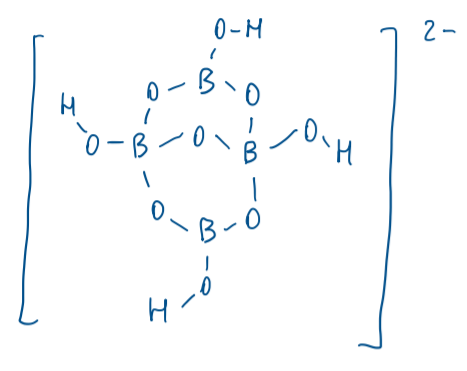
\includegraphics{images/11v7.png}

$Al_2O_3$

\textbf{Получение}

$$\gamma-Al(OH)_3 \xrightarrow{<400^{\circ}} Al_2O_3 + H_2O$$
$$Al + Cu_2O \xrightarrow{1000^{\circ}} Al_2O_3 + Cu$$
$$\gamma-Al_2O_3 \xrightarrow{>400^{\circ}} \alpha-Al_2O_3$$

\textbf{Химические свойства}

1) $\alpha-Al_2O_3$ - химически инертный

2) $\gamma-Al_2O_3$ - химически активный

$$\gamma-Al_2O_3 + H_2O + NaOH \rightarrow Na[Al(OH)_4(H_2O)_2]$$
$$\gamma-Al_2O_3 + H_2O + H_2SO_4 \rightarrow [Al(H_2O)_6]_2(SO_4)_3$$

Превращение в корунд

\textbf{Строение}

$\alpha-Al_2O_3,\rho = 4 \frac{g}{cm^3}$
Двухслойная плотнейшая шаровая упаковка из ионов О, в октаэдр. пустотах которой размещены ионы Al

$\gamma-Al_2O_3, \rho = 3,5 \frac{g}{cm^3}$ - кубическая форма

$AlO(OH), Al(OH)_3$

\textbf{Получение}

$$Al_2(SO_4)_3 + NH_3 + H_2O \rightarrow Al_2O_3\cdot xH_2O + (NH_3)_2SO_4$$

При старении $Al_2O_3\cdot xH_2O \rightarrow AlO(OH)$ - белит

$$Na[Al(OH)_4(H_2O)_2] + CO_2 \rightarrow Al(OH)_3\downarrow + NaHCO_3 + H_2O$$
(на холоде $\alpha-Al(OH)_3$ - байерит, в горячем растворе $\gamma-Al(OH)_3$ - гиббсит)

$$Al^{3+} + OH^- \rightarrow Al(OH)_3\downarrow$$

Взаимный гидролиз солей $Al^{3+}$ и солей с анионами $S^{2-}, SO_3^{2-}, CO_3^{2-}$

\textbf{Химические свойства}

$Al(OH)_3$ - амфотерный

$$Al(OH)_3 + KOH + H_2O \rightarrow K[Al(OH)_4(H_2O)_2]$$
$$Al(OH)_3 + KOH \xrightarrow{1000^{\circ}} KAlO_2 + H_2O$$
$$Al(OH)_3 \rightarrow Al_2O_3 + H_2O$$

$AlO(OH)$ - аналогично, но менее реакционноспособен

\textbf{Строение}

$\alpha-Al(OH)_3$ и $\gamma-Al(OH)_3$ - слоистые структуры, состоящие из связанных общими ребрами октаэдров $Al(OH)_6$

(Различие в способе образования стопок из слоев)

$AlO(OH)$ - стоистые структуры, состоящие из связанных общими ребрами октаэдров $Al(OH)_6$; н-связи

$\gamma-AlO(OH)$ - не плотнейшая упаковка

$Ga, In, Tl$

\textbf{Оксиды}

$Ga_2O_3$ - похож на $Al_2O_3$ по структуре и свойствам

$In_2O_3$ - собственный структурный тип ( кубический)

$Tl_2O$ - устойчивый, $Tl_2O_3$ - сильный окислитель

$$Tl_2O_3 \xrightarrow{100^{\circ}} Tl_2O + O_2$$
$$Tl_2O + H_2O \rightarrow TlOH$$
$$Tl(NO_3)_3 + KOH \rightarrow Tl_2O_3 + KNO_3 + H_2O$$
$$Tl_2O_3 + HCl \rightarrow TlCl\downarrow + H_2O + Cl_2\uparrow$$

\textbf{Гидроксиды}

$Ga(OH)_3$ - аналогичен по строение и свойстам $Al(OH)_3$\\
"идеальная" амфотерность : $pK_a = 6,8 ; pK_b  = 6,9$

$In(OH)_3$ - более сильное основание, чем $Al(OH)_3, Ga(OH)_3$

$TlOH$ - сильное основание, ведет себя подобно $OH^-$ ЩМ

$$Tl_2SO_3 + Ba(OH)_2 \rightarrow BaSO_4 +TlOH$$

$$Tl_2O = H_2O \rightarrow TlOH$$

$$TlOH + CO_2 \rightarrow Tl_2CO_3 + H_2O$$

$Tl(OH)_3$ крайне неустойчив

\subsubsection*{Галогениды}

$BX_3$

\textbf{Получение}

$BF_3$:

$$CaF_2 + Na_2B_4O_7 + H_2SO_4 \rightarrow BF_3 + NaHSO_4 + CaSO_4\downarrow + H_2O$$
$$B_2O_3 + NaBF_4 + H_2SO_{4(konc)} \rightarrow BF_3 + Na_2SO_4 + H_2O$$

$BCl_3, BBr_3$

$$B_2O_3 + C + X_2 \xrightarrow{700^{\circ}} CO + BX_3$$
$$AlX_3 + BF_3 \rightarrow BX_3 + AlF_3$$

-Прямой синтез

$BI_3$

$$LiBH_4 + I_2 \xrightarrow{-78^{\circ}} BI_3 + HI + LiI$$

\textbf{Химические свойства}

Сильные кислоты Льюиса, следовательно легко взаимодействуют с донорами электронов, например

$$BF_3 + HF \rightarrow H^+[BF_4]^-$$
$$BF_3 + Et_2O \rightarrow F_3B:OEt_2$$

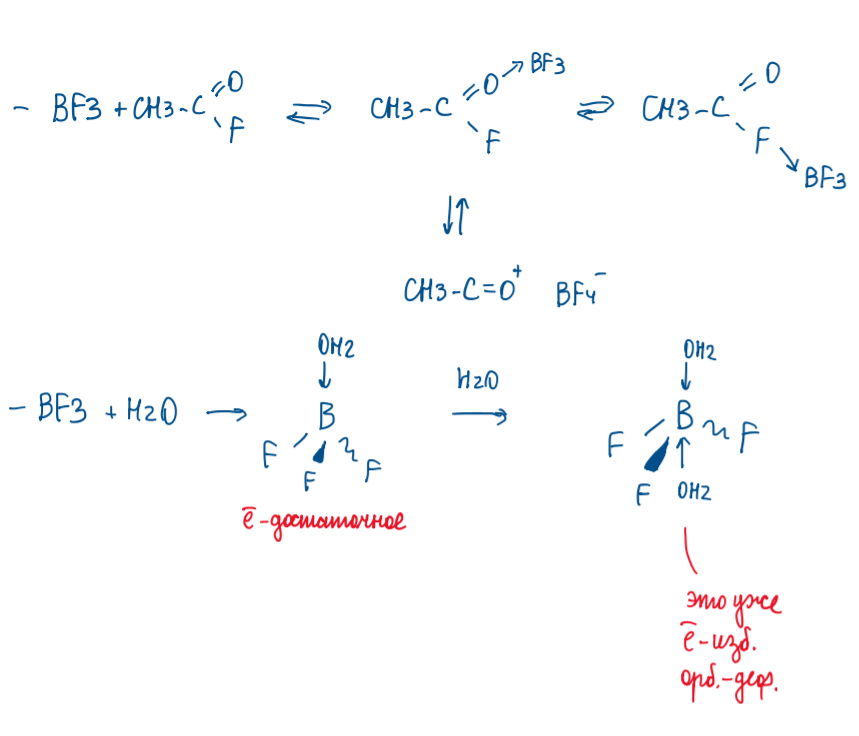
\includegraphics{images/11v8.png}

Гидролиз ($H_2O$ много, в отличие от прошлой реакции)

$$BF_3 + H_2O \rightarrow H_3BP_3 + HBF_4$$
$$BF_3 + H_2O \rightarrow BF_3\cdot 2H_2O (H_3O^+[F_3B:OH]^-)$$
$$BX_3 + H_2O \rightarrow H_3BO_3 + HX (X=Cl,Br,I)$$

\textbf{Строение}

В газовой фазе и в растворах - плоские ($D_{3h}$)\\
Могут быть неплоские в кристаллах

У B не 8, а 6 электронов, есть свободная p-орбиталь $\Rightarrow$ электроннодефицитные, орб. - избыточные

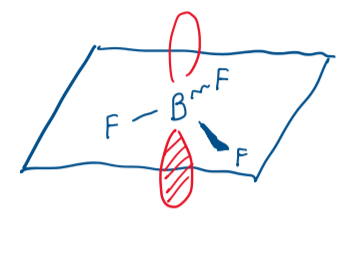
\includegraphics{images/11v9.png}

Мономерные соединения (но $BH_3$ - димер ($B_3H_6$))

При взаимодействии $BX_3$ и лиганда образуется тетраэдрическая структура,\\
Добавление лиганда ликвидирует электронодефицитность

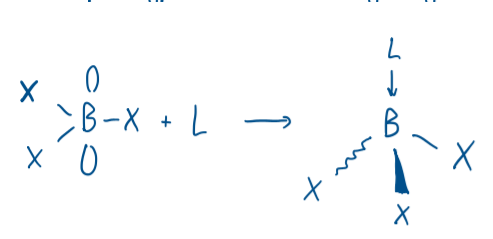
\includegraphics{images/11v10.png}

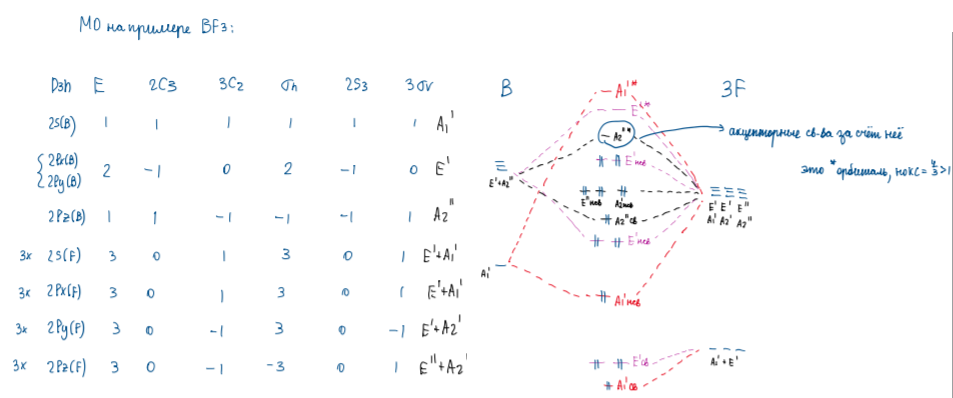
\includegraphics{images/11v11.png}


Существуют низшие галогениды:

$B_2X_2 (X=F,Cl,Br,I)$ и $B_nX_n (X = Cl, n = 4,7,12)$

Есть связь В-В

Малоустоййчивы, кроме $B_4Cl_3$
$$BCl_3 \rightarrow B_2Cl_4 + B_4Cl_4$$

$AlX, AlX_3$

\textbf{Получение}

Прямое воздействие

$$Al_2O_3 + C + Cl_2 \xrightarrow{600^{\circ}} AlCl_3 + CO$$

\textbf{Химические свойства}

Образует гидраты и комплексы 

$$AlCl_3 + 6H_2O \leftrightarrows [Al(H_2O)_6]^{3+} + 3Cl^-$$
$$AlCl_3 + Cl^- \xrightarrow{THF} AlCl_4^-$$
$$AlCl_3 + LiX \rightarrow AlX_3 + LiCl (X = Br, I)$$
$$AlCl_3 + LiY \rightarrow LiAlY + LiCl (Y=R,NH_2)$$

В газовой фазе есть AlX

В твердом состоянии неустойчивы

$$AlX \rightarrow Al + AlX_3$$

\textbf{Строение}

Образуют димеры $(AlX_3)_2$

Вообще Х может быть не только галоген, но и R или OR, т.к. тригалогенижы проявляют свойства кислот Льюиса.

$AlCl_3$:  К.Ч.(Al) = 6

Слои из  октаэдров $AlCl_6$, соед. общими ребрами $Al_2Cl_6$ устойчивы до $230^{\circ}$, выше - $AlCl_3$ 

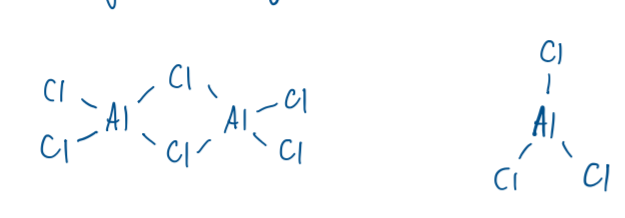
\includegraphics{images/11v12.png}

$AlX_3 (X= F, Br, I)$ - из молекул $Al_2X_6$, составленных их двух искаженных тетраэдров с общим ребром


$Ga, In, Tl$

Тригалогениды:

1) Все $MX_3$ (не $TlCl_3, TlBr_3, TlI_3$) синтезируют прямым взаимодействием или галогенированием оксидов

$$In + Cl_2 \xrightarrow{400^{\circ}} InCl_3$$

2) Получение $TlCl_3, TlI_3$

$$TlCl + NOCl \rightarrow TlCl_3 + NO$$
$$TlNO_3 + I_2 + HI \rightarrow TlI_3 + HNO_3$$

3) Не гидролизуются нацело, образуют гидраты, комплексы

$$K_3[InCl_6] \leftrightarrows 3K^+ + [InCl_6]^{3-}$$

4) $TlX_3$ - сильные окислители

$$TlCl_3 + Na_2S \rightarrow Tl_2S + S + NaCl$$
$$TlCl_3 + FeCl_2 \rightarrow FeCl_3 + TlCl$$

5) $TlX_3$ - легко разлагаются при нагревании

$$TlCl_3 \xrightarrow{153^{\circ}} TlCl + Cl_2$$
$$TlBr_3 \xrightarrow{\approx 40^{\circ}} Tl_2Br_4 + Br_2$$

Низшие галогениды:

1) Все MX известны (кроме $GaF, InF$)

2) Только $TlF$ хорошо растворим в воде

3) $GaX, InX$ диспропорционируют при нагревании
$$GaI \rightarrow GaI_3 + Ga$$

4) $TlX$ - устойчивые ионные галогениды, аналогично ЩМ

5) $TlX, InI$ не гидролизуется

6) у $TlX$ нет устойчивых комплексов

$$TlCl + NH_3\cdot H_2O \nrightarrow$$

7) Известны $M_2X_4$ $M[MX_4]$

$TlF$ - структура $NaCl$

$TlCl, ClBr, TlI$ - структура $CsCl$
